\begin{figure}[H]
    \centering

    \tikzset{
    max node/.style={circle,draw,inner sep=5},
    min node/.style={circle,draw,inner sep=5, fill=gray}
    }

    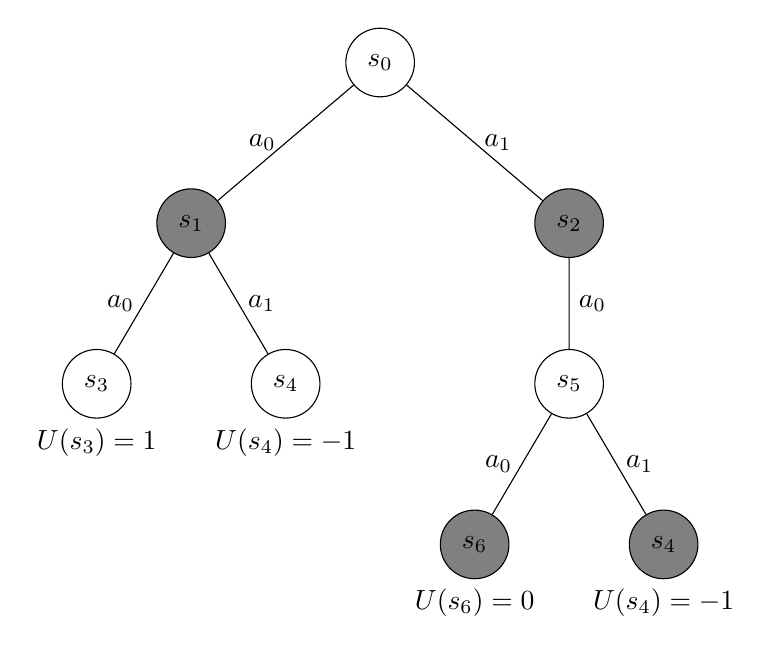
\begin{tikzpicture}[scale=12]
    % Specify spacing for each level of the tree
    \tikzstyle{level 1}=[level distance=1.7mm,sibling distance=4mm]
    \tikzstyle{level 2}=[level distance=1.7mm,sibling distance=2mm]
    % The Tree
    \node(0)[max node]{$s_0$}
    child{node(1)[min node]{$s_1$}
        child{node[max node, label=below:{$U(s_3)=1$}]{$s_3$}
            edge from parent node[left]{$a_0$}
        }
        child{node[max node, label=below:{$U(s_4)=-1$}]{$s_4$}
            edge from parent node[right]{$a_1$}
        }
        edge from parent node[left]{$a_0$}
    }
    child{node(2)[min node]{$s_2$}
        child{node[max node]{$s_5$}
            child{node[min node, label=below:{$U(s_6)=0$}]{$s_6$}
                edge from parent node[left]{$a_0$}
            }
            child{node[min node, label=below:{$U(s_4)=-1$}]{$s_4$}
                edge from parent node[right]{$a_1$}
            } 
            edge from parent node[right]{$a_0$}
        }
        edge from parent node[right]{$a_1$}
    };

    \end{tikzpicture}

    \caption{A simple game tree where white nodes correspond to the
    Max player's turn, and grey nodes to the Min player's. Notice how
    not all actions are applicable in all states, terminal states do
    not have to be on the same depth, and a given terminal state will have
    the same utility regardless of the path leading to it.}
    \label{fig:game_tree}

\end{figure}
